\documentclass[11pt]{article}
\usepackage{amsmath, amssymb, amsthm}

\usepackage[pdftex]{graphicx}

\usepackage{fancyhdr}
%Format stuff
\pagestyle{fancy}
\headheight 35pt

%Header info
\chead{\Large \textbf{Minimal Spanning Trees}}
\lhead{}
\rhead{}

\begin{document}
	A minimum spanning tree (MST) for a connected graph $G = (V, E)$ is an acyclic subset of edges that spans all vertices with minimum total edge weight.
	
	In general, MST's have the following properties:
	\begin{itemize}
		\item $n$ nodes on $n - 1$ edges
		\item Adding an edge introduces a cycle
		\item Removing any edge in such a cycle restores the spanning tree
	\end{itemize}

Given a cut $(S, V - S)$, it respects a subset of edges if none of those edges crosses the cut.

\subparagraph{Claim} If $(S, V - S)$ is any cut that respects some viable MST solution denoted as a set of edges $A$, then the lightest edge that crosses this cut is always "safe" to add.

\subparagraph{Proof} By contradiction, imagine 2 cuts of a part of a viable solution that we add a non-minimum crossing edge to:

	\begin{figure}[htb]
		\centering
		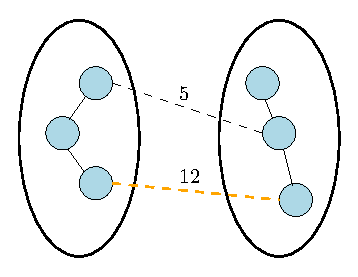
\includegraphics{mst-safe-cut.eps}
		\label{fig:figure}
	\end{figure}
	However, we can swap out the expensive edge for a cheaper crossing edge and still maintain a spanning tree with lower weight, so therefore the lightest crossing edge is always a safe edge to add. Call this the \textbf{safe edge lemma}


%	\begin{center}
%	\begin{tikzpicture}
%		[scale=3,line cap=round,
%		%Styles
%		axes/.style=,
%		important line/.style={very thick},
%		information text/.style={rounded corners,fill=red!10,inner sep=1ex},
%		dot/.style={circle,inner sep=1pt,fill,label={#1},name=#1}			
%		]
%		
%		%Colors
%		\colorlet{anglecolor}{green!50!black}	%angle arcs/lines
%		
%		%The graphic
%	\end{tikzpicture}
%	\end{center}


%		\def\enotesize{\normalsize}
%		\theendnotes
\end{document}